% Created 2010-08-17 Tue 13:49
\documentclass{article}
\usepackage{graphicx}
\usepackage{times}
\usepackage[margin=0.75in]{geometry}


\title{Inserting an AHIR module in the NetFPGA framework}
\author{Madhav Desai}

\begin{document}

\maketitle

\section{Overview}

This document describes the mechanism by which an 
AHIR generated VHDL system can be included in the NetFPGA packet
processing implementation framework.  

The AHIR generated VHDL system is required to fit into 
a NetFPGA user-module template. It is relatively easy to
achieve this. 


\section{Mechanism}

The user module template has the form shown in Figure \ref{fig:NetFPGAUserModule}.
\begin{figure}
  \centering
  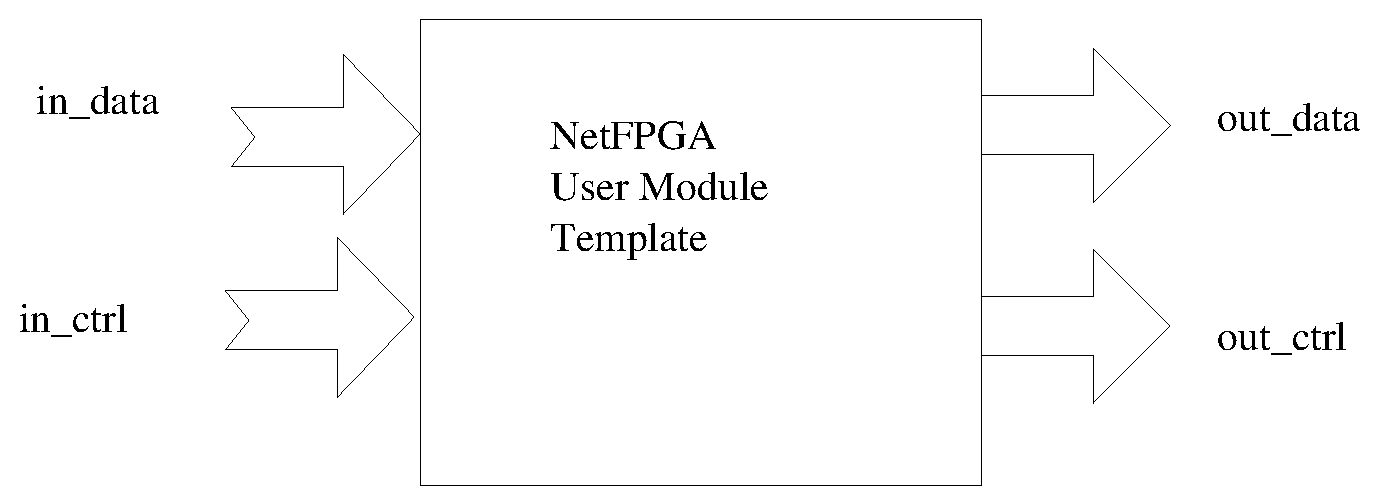
\includegraphics[scale=0.7]{NetFPGAUserModule.eps}
  \caption{NetFPGA User Module}
  \label{fig:NetFPGAUserModule}
\end{figure}
The interface is very simple: an input data and control bus,
and an output data and control bus.

A generic AHIR system can have the form shown in Figure \ref{fig:GenericAhirSystem}.
\begin{figure}
  \centering
  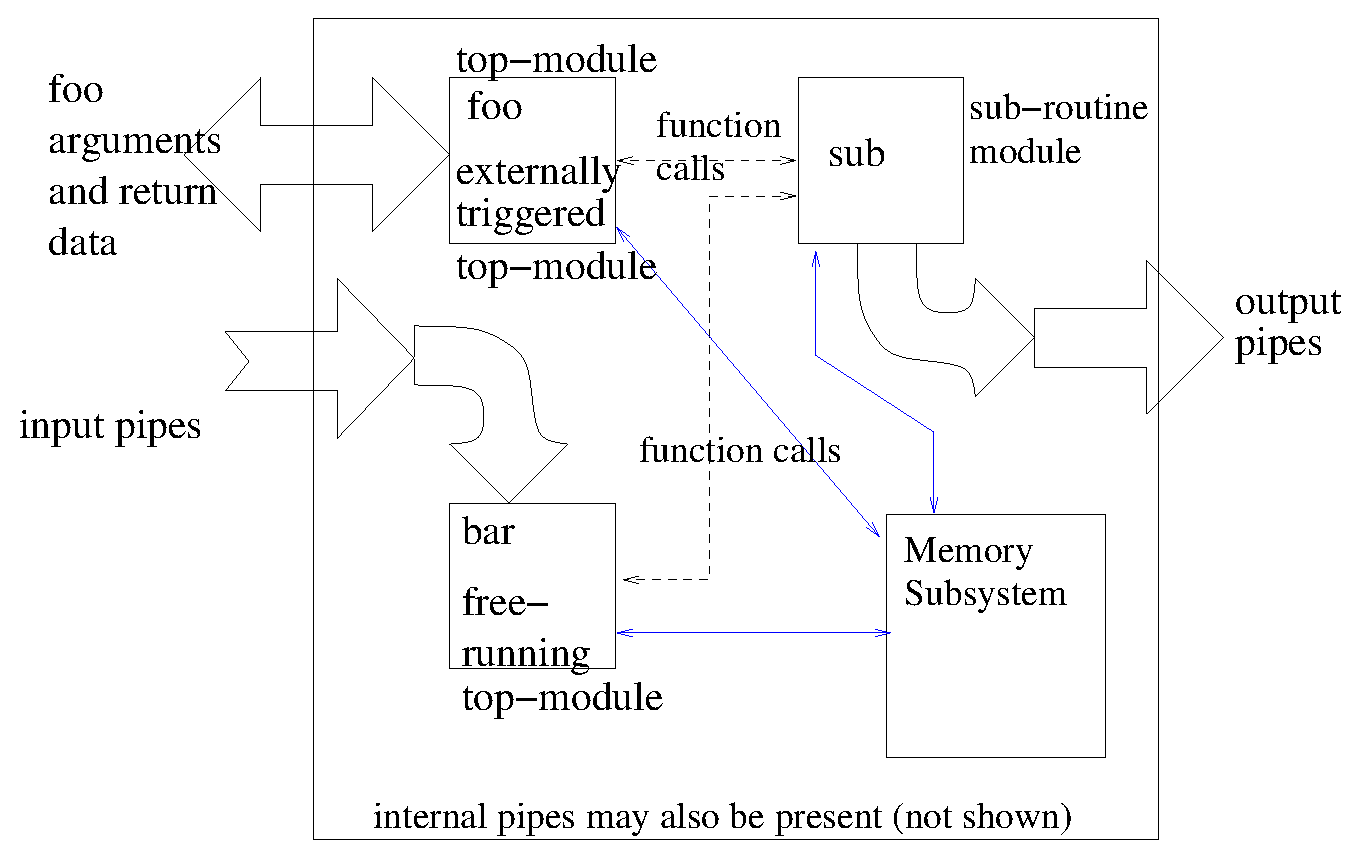
\includegraphics[scale=0.7]{GenericAhirSystem.eps}
  \caption{Generic AHIR system}
  \label{fig:GenericAhirSystem}
\end{figure}



In order to insert a generic AHIR system into a NetFPGA user-module template:
\begin{itemize}
\item we ensure that the only interaction of the AHIR system with the outside world is
through four pipes: two input pipes for the input data and control, and
two output pipes for the output data and control.
\item The top-level modules in the AHIR system are free-running.  
The set of modules (functions) are of two kinds.  The first
kind consists of functions generated from the click to llvm to AHIR
flow.  The second kind consists of three fixed free-running modules:
two free-running modules which are 
responsible for interactions with the outside world (through the four pipes
discussed above) and a third free-running module which manages a packet-queue.
\begin{itemize}
\item an input-module which will collect data from the input pipes and
forward to appropriate pipes/modules in the AHIR system.
\item an output-module which will collect data from internal pipes/modules
in the AHIR system and forward it to the the system output pipes.
\item a free-queue-manager which provides packet slots to the input-module
and receives empty packet slots from the output-module.
\end{itemize}
\item The AHIR system would be instantiated in a {\em fixed} wrapper
which would be responsible for the protocol matching between the AHIR
system interface and the NetFPGA user module interface.
\end{itemize}


\section{Issues: memory management}

One issue that needs to be resolved is that of memory management.
This relates to two processes:
\begin{itemize}
\item Initialization: must be explicitly done in 
the source program.
\item Exchange of information between the AHIR memory subsystem and
the outside world:  If this is needed, it would need to be explicitly 
built into the input/output modules.  Note that an exchange of
information (in general) may be initiated from ``inside'' or
from ``outside'' the AHIR system.
\end{itemize}

\section{Implementation}

The process of including the AHIR system in a NetFPGA user template is
exactly the same as that of verifying an AHIR system using a C-testbench
with the assumption that the testbench only sends/receives packets to the AHIR 
system.  Most of the basic infrastructure for this is in place.  The only
necessary components are the input and output modules outlined in the 
previous section.

Originally, Sameer had implemented the input and output module for
a specific scenario (as documented in the previous plan).  In this
scenario, the input module would receive the data from the NetFPGA
surroundings, would put the data packet into a free memory slot and would trigger
the AHIR module.  On completion of the AHIR module, the output module
would take the modified data from memory and would forward it to
the NetFPGA environment.   The memory slots would be organized into
a queue emptied by the input module and filled by the output module.

What would be easiest, in my opinion would be
\begin{itemize}
\item use the parts of Sameer's code that do the protocol
translation (between the NetFPGA user-module and an AHIR module).
\begin{itemize}
\item we re-implement a VHDL entity {\em netfpga\_module} which 
would instantiate an AHIR system with four interface pipes (see Figure \ref{fig:NetFpgaAhirSystemWrap}).
\begin{figure}
  \centering
  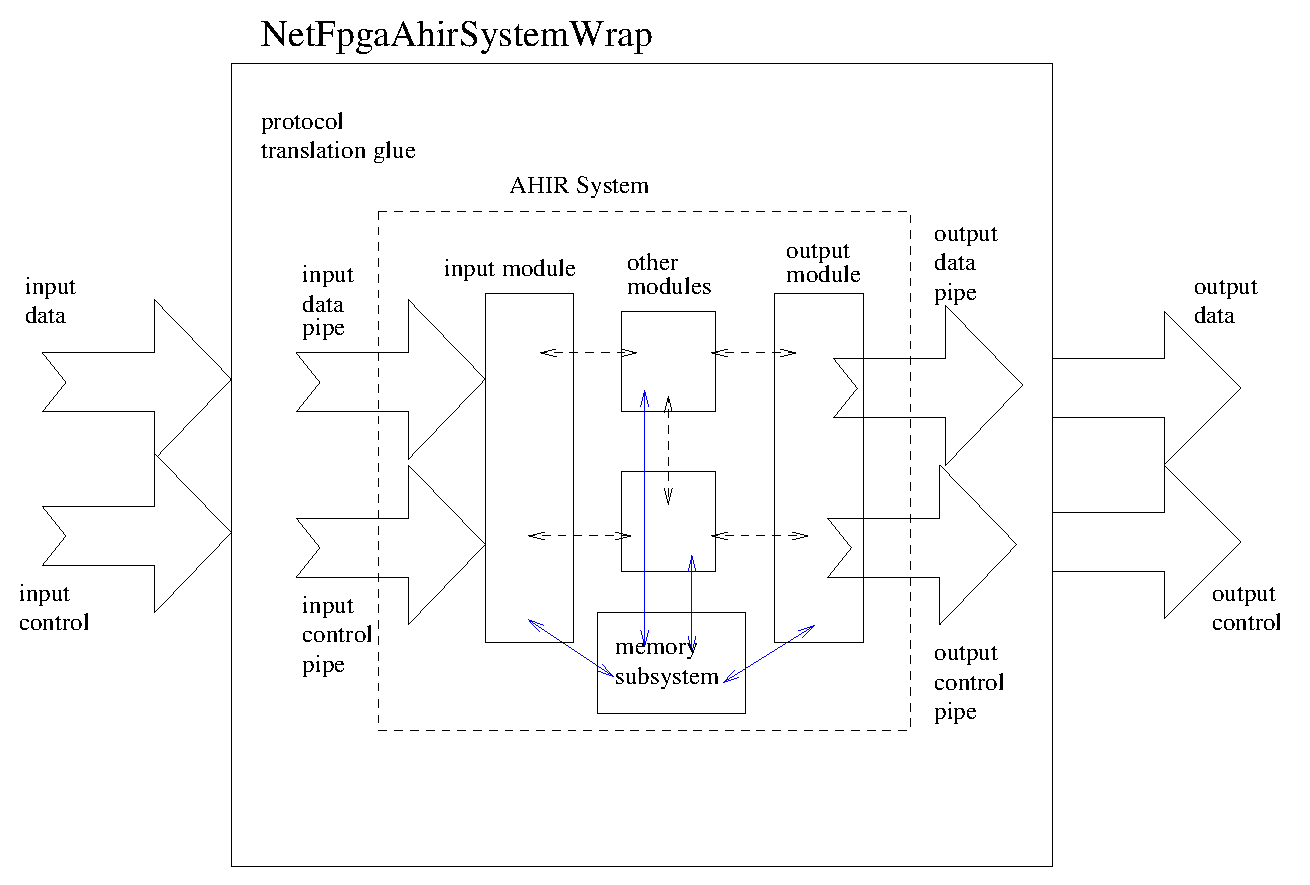
\includegraphics[scale=0.7]{NetFpgaAhirSystemWrap.eps}
  \caption{NetFpgaAhirSystemWrap Schematic}
  \label{fig:NetFpgaAhirSystemWrap}
\end{figure}
\end{itemize}
\item write the input and output modules and
a free queue manager in C and add them 
to the AHIR flow to generate the final AHIR system. 
\begin{itemize}
\item This can be written for
the specific system being generated.  Note that we will have
to pay some attention to memory initialization and transfer of
information between the AHIR memory subsystem and the outside
world.  I have done a reference implementation based on
Sameer's VHDL code.  This needs to be reviewed.
\end{itemize}
\item generate the final AHIR system by including the input/output modules
written in C.  This is easiest to do by linking the llvm byte-code for
the input/output modules with the click2llvm generated byte-code.
\item Instantiate the final AHIR system in a netfpga pipeline module.
\end{itemize}
The process is indicated in Figure \ref{fig:Wrap}.   


\begin{figure}
  \centering
  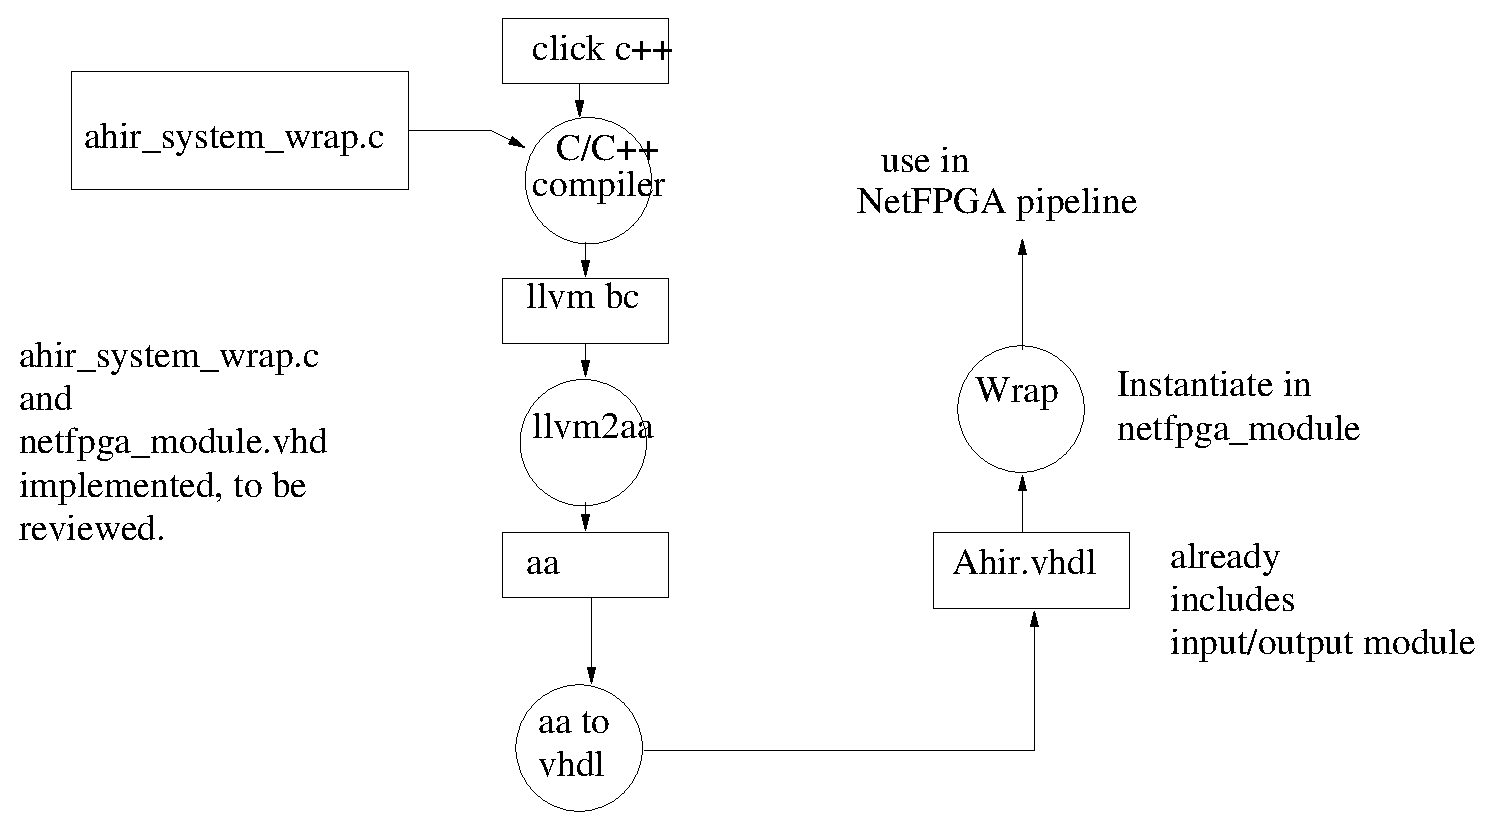
\includegraphics[scale=0.7]{NetFPGAWrap.eps}
  \caption{NetFPGA Wrap Flow}
  \label{fig:Wrap}
\end{figure}

In the folders AHIRGIT/ericsson/C and AHIRGIT/ericsson/vhdl,
I have put an implementation of the C source (input/output module, free-queue
manager) and the netfpga-wrapper module.  The C source implements
Sameer's input module, output module and free queue manager (this should
be linked with the click2llvm stuff during the AHIR compile chain).
The vhdl is a very simple wrapper which just does protocol
translation. 




\end{document}
